\begin{figure}[ht]
\centering
\begin{subfigure}[t]{0.98\textwidth}
  \centering
  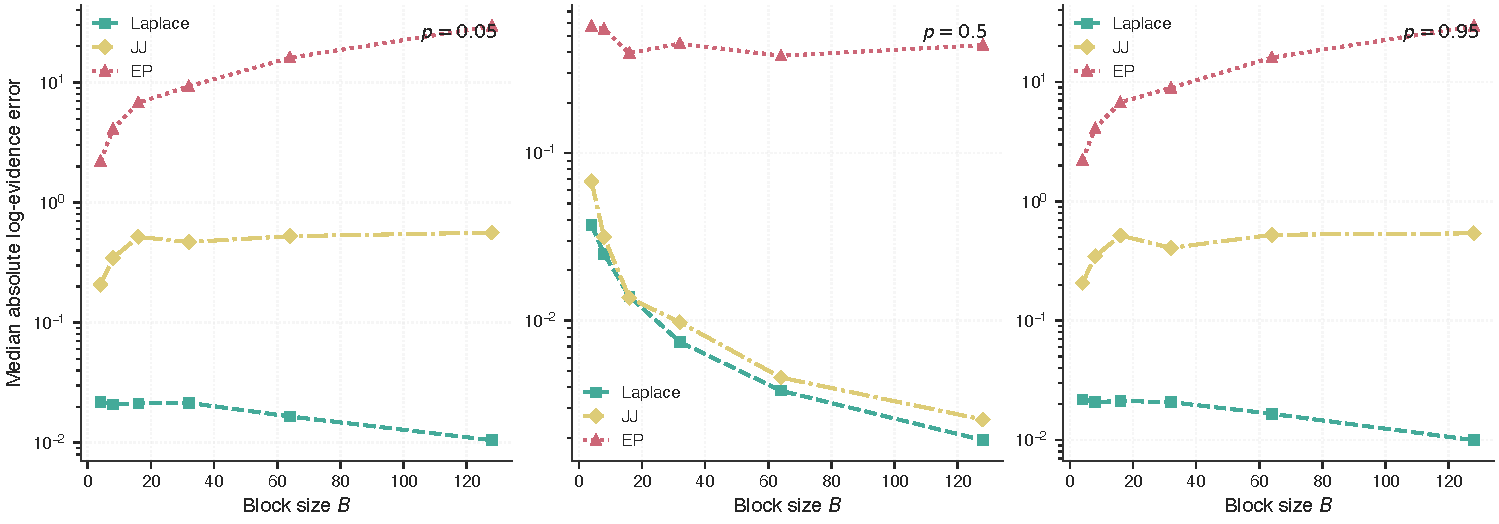
\includegraphics[width=\textwidth]{figures/fig_E06_local_error}
  \caption{Median absolute log-evidence error by block size $B$ and generating success probability
  $p$. Laplace errors are small (median $|\Delta\log Z|=0.021$, max $0.038$) and decrease
  with $B$ at balanced $p$. JJ errors are uniformly negative (lower bound) with median
  $0.22$ and maximum $0.98$; errors are larger at extreme $p$ values. EP errors are large
  (median $3.78$, max $30.0$) and systematically positive for extreme $p$, reflecting
  that parallel EP is not a guaranteed lower bound on the log-marginal.}
  \label{fig:e06-local-error}
\end{subfigure}

\vspace{1em}

\begin{subfigure}[t]{0.98\textwidth}
  \centering
  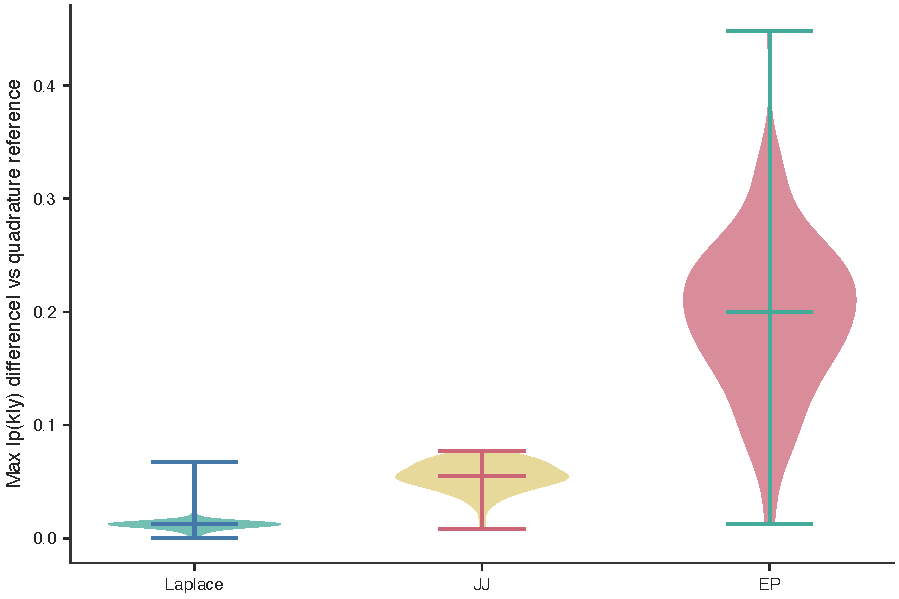
\includegraphics[width=\textwidth]{figures/fig_E06_global_error}
  \caption{Segmentation propagation discrepancies versus the quadrature reference
  ($n=96$, $k_{\rm true}=3$, boundaries at $(32,64)$, 100 independent sequences).
  Laplace: mean max $|p(k|y)|$ difference $0.013$, 1 MAP mismatch. JJ: mean $0.056$,
  19 MAP mismatches. EP: mean $0.236$, 89 MAP mismatches.
  EP boundary-marginal discrepancies reach $0.84$ in individual sequences.}
  \label{fig:e06-global-error}
\end{subfigure}

\caption{Experiment E06: local and global effects of nonconjugate block-evidence
approximations. (a) Absolute log-evidence error by block size and success probability.
(b) Count posterior and boundary-marginal discrepancies in the segmentation propagation
experiment. Reference in both panels is mode-centred adaptive quadrature
($\texttt{epsabs}=10^{-12}$).}
\label{fig:planned-nonconjugate-paper}
\end{figure}
